\documentclass[tikz,border=10pt]{standalone}
\usepackage{tikz}
\usepackage{fontawesome5}
\usepackage{amsmath,amssymb}
\usetikzlibrary{arrows.meta,positioning,fit,backgrounds,calc,shadows,shapes.geometric}

% Color definitions
\definecolor{lavenderDark}{RGB}{15, 44, 89}
\definecolor{lavenderDeep}{RGB}{10, 28, 58}
\definecolor{lavenderMedium}{RGB}{29, 78, 158}
\definecolor{lavenderLight}{RGB}{240, 246, 255}
\definecolor{lavenderBorder}{RGB}{180, 205, 237}
\definecolor{prismNavy}{RGB}{15, 44, 89}
\definecolor{prismBlue}{RGB}{29, 78, 158}
\definecolor{prismTeal}{RGB}{13, 148, 136}
\definecolor{prismGold}{RGB}{217, 119, 6}
\definecolor{prismDark}{RGB}{15, 23, 42}
\definecolor{prismSlate}{RGB}{100, 116, 139}
\definecolor{statusFail}{RGB}{220, 38, 38}
\definecolor{cInput}{RGB}{241, 245, 249}
\definecolor{cStem}{RGB}{224, 242, 254}
\definecolor{cStage1}{RGB}{209, 250, 229}
\definecolor{cStage2}{RGB}{254, 243, 199}
\definecolor{cStage3}{RGB}{254, 226, 226}
\definecolor{cStage4}{RGB}{207, 250, 254}
\definecolor{cHead}{RGB}{219, 234, 254}

\begin{document}
% CoMViT Architecture Decomposition and Layer Connectivity Graph
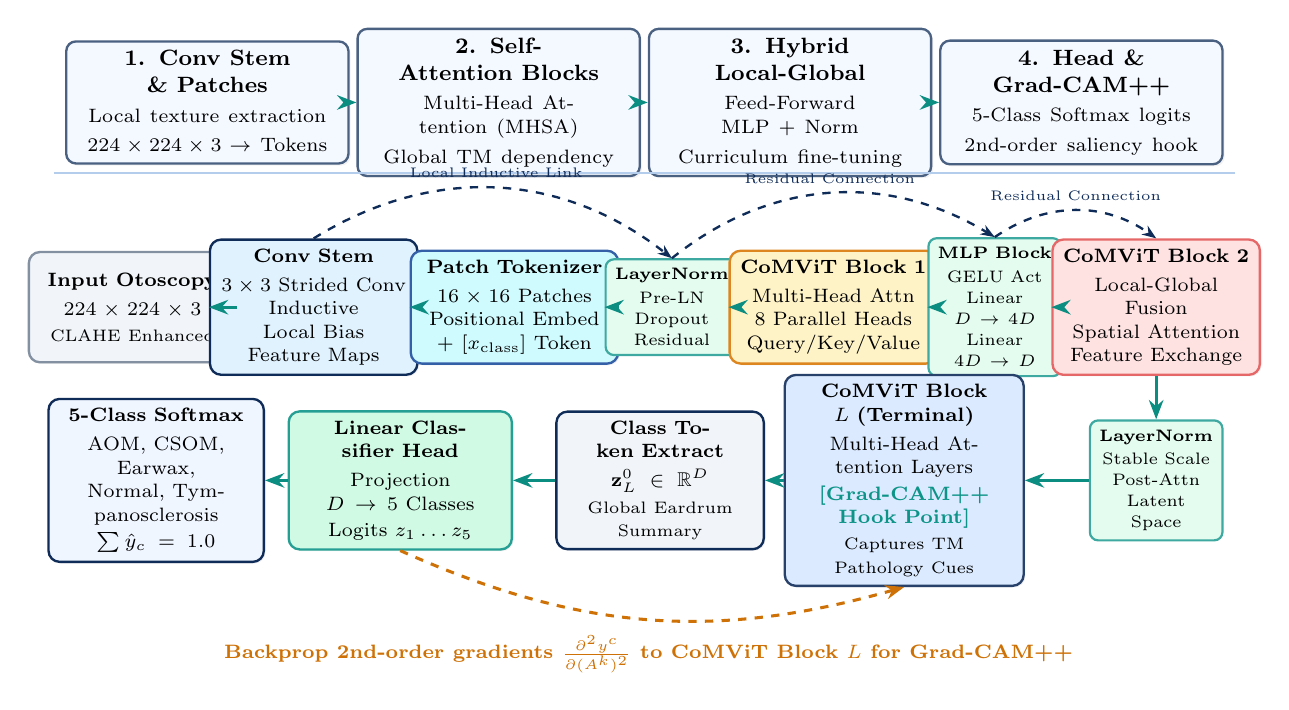
\begin{tikzpicture}[
  x=1cm, y=1cm,
  font=\sffamily,
  dagstep/.style={rectangle, rounded corners=3.5pt, minimum height=1.10cm,
    text width=3.35cm, align=center, draw=lavenderDark!75, fill=lavenderLight!75,
    line width=0.85pt, font=\fontsize{8.2}{9.8}\selectfont\bfseries,
    drop shadow={shadow xshift=0.8pt, shadow yshift=-0.8pt, opacity=0.10}},
  dagarrow/.style={-{Stealth[scale=0.85]}, line width=1.15pt, draw=prismTeal!95!black},
  blkbox/.style={rectangle, rounded corners=4pt, line width=0.85pt,
    minimum height=1.40cm, text width=2.40cm, align=center,
    font=\fontsize{7.2}{8.5}\selectfont, drop shadow={shadow xshift=0.6pt, shadow yshift=-0.6pt, opacity=0.12}},
  transbox/.style={rectangle, rounded corners=3pt, line width=0.80pt,
    draw=prismTeal!80, fill=cStage1!60, minimum height=1.15cm, text width=1.45cm, align=center,
    font=\fontsize{6.5}{7.6}\selectfont},
  skipconn/.style={-{Stealth[scale=0.75]}, line width=0.85pt, draw=prismNavy, dashed}
]

  % Row 1: 4-Stage Architectural Progression
  \node[dagstep] (s1) at (-5.55, 0) {1. Conv Stem \& Patches\\[2pt]\normalfont\fontsize{7.2}{8.5}\selectfont Local texture extraction\\[1pt]$224\times 224\times 3 \to$ Tokens};
  \node[dagstep] (s2) at (-1.85, 0) {2. Self-Attention Blocks\\[2pt]\normalfont\fontsize{7.2}{8.5}\selectfont Multi-Head Attention (MHSA)\\[1pt]Global TM dependency};
  \node[dagstep] (s3) at (1.85, 0) {3. Hybrid Local-Global\\[2pt]\normalfont\fontsize{7.2}{8.5}\selectfont Feed-Forward MLP + Norm\\[1pt]Curriculum fine-tuning};
  \node[dagstep] (s4) at (5.55, 0) {4. Head \& Grad-CAM++\\[2pt]\normalfont\fontsize{7.2}{8.5}\selectfont 5-Class Softmax logits\\[1pt]2nd-order saliency hook};

  \draw[dagarrow] (s1) -- (s2);
  \draw[dagarrow] (s2) -- (s3);
  \draw[dagarrow] (s3) -- (s4);

  % Separator
  \draw[draw=lavenderBorder, line width=0.6pt] (-7.5, -0.90) -- (7.5, -0.90);

  % Row 2 & 3: Detailed Layer Decomposition Flow
  \node[blkbox, fill=cInput, draw=prismSlate!80] (input_node) at (-6.50, -2.60) {
    \textbf{Input Otoscopy}\\[2pt]
    $224\times 224\times 3$\\[1pt]
    {\fontsize{6.0}{7.0}\selectfont CLAHE Enhanced}
  };

  \node[blkbox, fill=cStem, draw=lavenderDark] (stem_node) at (-4.20, -2.60) {
    \textbf{Conv Stem}\\[2pt]
    $3\times 3$ Strided Conv\\
    Inductive Local Bias\\
    Feature Maps
  };

  \node[blkbox, fill=cStage4, draw=prismBlue!90] (token_node) at (-1.65, -2.60) {
    \textbf{Patch Tokenizer}\\[2pt]
    $16\times 16$ Patches\\
    Positional Embed\\
    + $[x_{\text{class}}]$ Token
  };

  \node[transbox] (tr1) at (0.35, -2.60) {
    \textbf{LayerNorm}\\[1pt]
    Pre-LN\\
    Dropout\\
    Residual
  };

  \node[blkbox, fill=cStage2, draw=prismGold!90] (vit1) at (2.40, -2.60) {
    \textbf{CoMViT Block 1}\\[2pt]
    Multi-Head Attn\\
    8 Parallel Heads\\
    Query/Key/Value
  };

  \node[transbox] (tr2) at (4.45, -2.60) {
    \textbf{MLP Block}\\[1pt]
    GELU Act\\
    Linear $D\to 4D$\\
    Linear $4D\to D$
  };

  \node[blkbox, fill=cStage3, draw=statusFail!70] (vit2) at (6.50, -2.60) {
    \textbf{CoMViT Block 2}\\[2pt]
    Local-Global Fusion\\
    Spatial Attention\\
    Feature Exchange
  };

  % Second Row of Layers
  \node[transbox] (tr3) at (6.50, -4.80) {
    \textbf{LayerNorm}\\[1pt]
    Stable Scale\\
    Post-Attn\\
    Latent Space
  };

  \node[blkbox, fill=cHead, draw=lavenderDark!90, text width=2.80cm] (vitL) at (3.30, -4.80) {
    \textbf{CoMViT Block $L$ (Terminal)}\\[2pt]
    Multi-Head Attention Layers\\[1pt]
    {\color{prismTeal}\textbf{[Grad-CAM++ Hook Point]}}\\[1pt]
    {\fontsize{6.0}{7.0}\selectfont Captures TM Pathology Cues}
  };

  \node[blkbox, fill=cInput, draw=prismNavy] (cls_token) at (0.20, -4.80) {
    \textbf{Class Token Extract}\\[2pt]
    $\mathbf{z}_L^0 \in \mathbb{R}^D$\\[1pt]
    {\fontsize{6.0}{7.0}\selectfont Global Eardrum Summary}
  };

  \node[blkbox, fill=cStage1, draw=prismTeal!90, text width=2.60cm] (head) at (-3.10, -4.80) {
    \textbf{Linear Classifier Head}\\[2pt]
    Projection $D \to 5$ Classes\\[1pt]
    Logits $z_1 \dots z_5$
  };

  \node[blkbox, fill=lavenderLight, draw=lavenderDark, text width=2.50cm] (softmax) at (-6.20, -4.80) {
    \textbf{5-Class Softmax}\\[2pt]
    AOM, CSOM, Earwax,\\
    Normal, Tympanosclerosis\\[1pt]
    $\sum \hat{y}_c = 1.0$
  };

  % Forward Flow Connections
  \draw[dagarrow] (input_node) -- (stem_node);
  \draw[dagarrow] (stem_node) -- (token_node);
  \draw[dagarrow] (token_node) -- (tr1);
  \draw[dagarrow] (tr1) -- (vit1);
  \draw[dagarrow] (vit1) -- (tr2);
  \draw[dagarrow] (tr2) -- (vit2);
  \draw[dagarrow] (vit2) -- (tr3);
  \draw[dagarrow] (tr3) -- (vitL);
  \draw[dagarrow] (vitL) -- (cls_token);
  \draw[dagarrow] (cls_token) -- (head);
  \draw[dagarrow] (head) -- (softmax);

  % Skip Connections
  \draw[skipconn] (stem_node.north) to[bend left=35] node[above, font=\fontsize{5.5}{6.5}\selectfont\color{prismNavy}]{Local Inductive Link} (tr1.north);
  \draw[skipconn] (tr1.north) to[bend left=35] node[above, font=\fontsize{5.5}{6.5}\selectfont\color{prismNavy}]{Residual Connection} (tr2.north);
  \draw[skipconn] (tr2.north) to[bend left=35] node[above, font=\fontsize{5.5}{6.5}\selectfont\color{prismNavy}]{Residual Connection} (vit2.north);

  % Backward Hook Arrow
  \draw[-{Stealth[scale=0.85]}, line width=1.1pt, draw=prismGold!95!black, dashed] 
    (head.south) to[bend right=20] 
    node[below=2pt, font=\fontsize{6.8}{8.0}\selectfont\bfseries\color{prismGold!95!black}]{Backprop 2nd-order gradients $\frac{\partial^2 y^c}{\partial (A^k)^2}$ to CoMViT Block $L$ for Grad-CAM++} 
    (vitL.south);

\end{tikzpicture}
\end{document}
